\section{一个例子和待完成}

\subsection{目前正在 debug 的液柱垮塌算例}

% \begin{frame}
%     考虑一个液柱(可以认为是玻璃杯的水,在某时刻撤去所有杯壁)。
%     以下可视化是基于 pyvista 的,可以看到,液柱在撤去杯壁后,开始垮塌。
    
%     \begin{figure}[H]
%         \includegraphics[width=0.8\textwidth]{image/step1.png}
%         \caption{液柱垮塌算例时刻 0}
%     \end{figure}

% \end{frame}

% \begin{frame}
%     \begin{figure}[H]
%         \includegraphics[width=0.8\textwidth]{image/step6.png}
%         \caption{液柱垮塌算例时刻 0.06}
%     \end{figure}

% \end{frame}

% \begin{frame}
%     \begin{figure}[H]
%         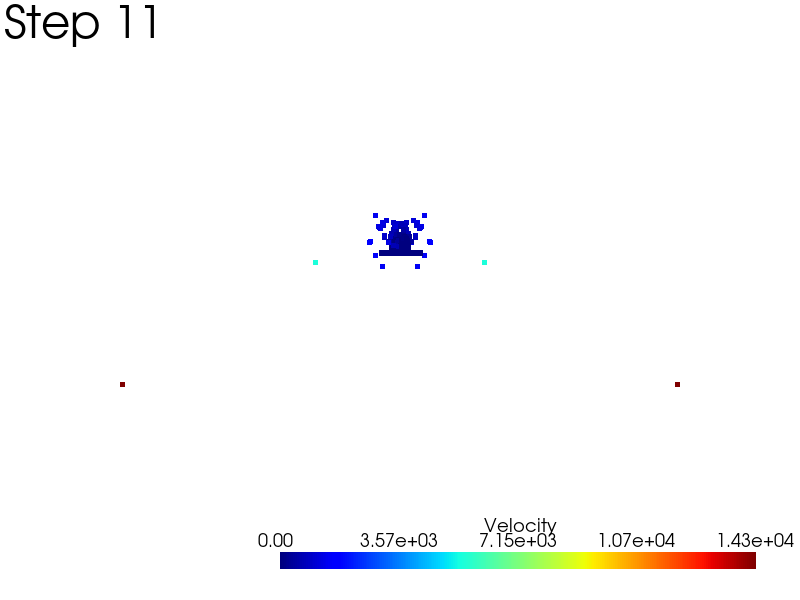
\includegraphics[width=0.8\textwidth]{image/step11.png}
%         \caption{液柱垮塌算例时刻 0.11}
%     \end{figure}
% \end{frame}

% \begin{frame}
%     \begin{figure}[H]
%         \includegraphics[width=0.8\textwidth]{image/step16.png}
%         \caption{液柱垮塌算例时刻 0.16}
%     \end{figure}
% \end{frame}

% \begin{frame}
%     \begin{figure}[H]
%         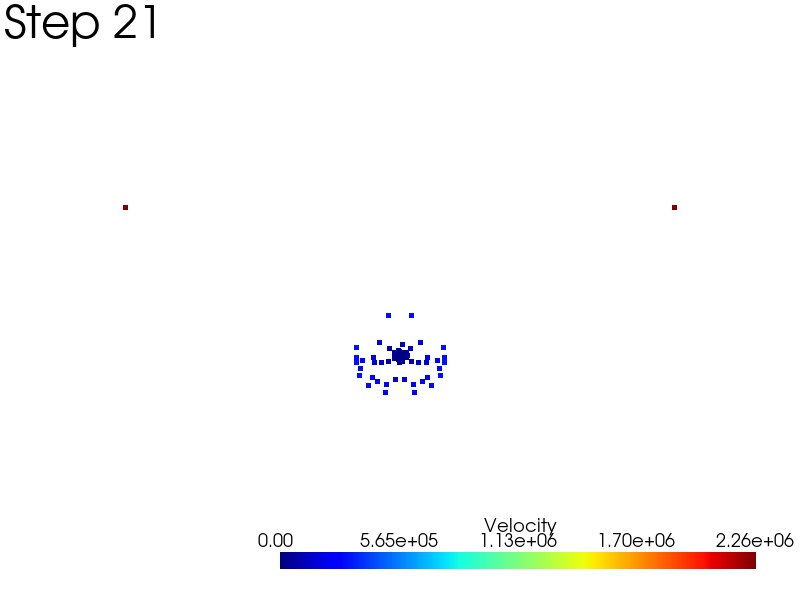
\includegraphics[width=0.8\textwidth]{image/step21.png}
%         \caption{液柱垮塌算例时刻 0.21}
%     \end{figure}
% \end{frame}

% \begin{frame}
%     \begin{figure}[H]
%         \includegraphics[width=0.8\textwidth]{image/step26.png}
%         \caption{液柱垮塌算例时刻 0.26}
%     \end{figure}
% \end{frame}

% \begin{frame}
%     \begin{figure}[H]
%         \includegraphics[width=0.6\textwidth]{image/step31.png}
%         \caption{液柱垮塌算例时刻 0.31}
%     \end{figure}

%     在第 0.31 时刻,液柱开始有点崩坏,
%     不清楚是数值格式中哪块出了问题。
%     目前可以肯定的是,
%     边界条件的处理是有问题的。
%     但在目前的程序结构下不知道采用什么别的格式好做一些。
% \end{frame}

\subsection{待完成的工作}

\begin{frame}
    \begin{itemize}
        \item 修复边界条件处理
        \item 检验核函数插值的正确性
        \item 尝试不可压缩的 SPH 数值格式
        \item 快速粒子搜索算法*(这点很重要,会影响到后面的工作)
    \end{itemize}
\end{frame}